\section{Optical Flow}
\label{sec:bg_opticalflow}
Optical Flow is the motion of objects revealed in image sequences or videos~\cite{fleet2006optical},\cite{Sun2010}. By estimating optical flow between frames in video sequences, motion, translation, deformation and many feature can be revealed. Optical flow is applicable under specific assumptions:
\begin{itemize}
  \item Motion of objects is smooth and gradually over time.
  \item Illumination is relatively consistent in given sequence. To be more specific, the pixel measurement in a small region remain the same despite of location changes.
\end{itemize}
A flow between two consecutive frames defines pixel movement from former frame to later frame. Defining former frame as \(I_n(i,j)\) where \(i,j\) represent pixel coordinate, the later frame is defined as \(I_{n+1}(i+u_{i,j},j+v_{i,j})\) where \(u_{i,j},v_{i,j}\) are horizontal and vertical translation of pixel (\(i,j\)). The fundamental algorithm of optimal optic flow is find a set of $u, v$ (flow directions) that minimised the objective error function:
\begin{equation}
E(p)=\sum^f_{n=1}\sum^{p}_{i,j\in p}[I_n(i,j)-I_{n+1}(i+u_{i,j},j+v_{i,j})]+regularisation
\end{equation}
where $f$ is number of frames in target sequence, $p$ is set of pixels in frame. Generally the error function contains a regularization term to prevent over fitting. Recent researches also suggest appending subspace constrains to error function~\cite{Garg2013, Garg, Garg2013a}. 

\begin{figure}[ht]
\centering
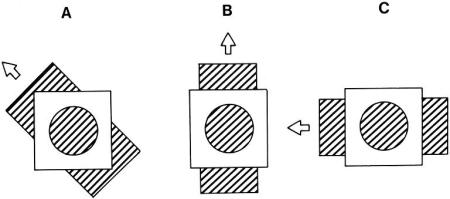
\includegraphics[width=0.9\textwidth]{resources/Background/aperture_problem}
\caption{Aperture Problem}
\label{fig:aperture_problem}
\end{figure}

\subsection{Aperture Problem}

Optical flow suffers from Aperture Problem. the aperture problem occur when determine global motion of objects from a small fraction of observation field. Figure \ref{fig:aperture_problem} demonstrate a situation when aperture problem occurs. Squares A, B and C all having different motion direction. But from only the circle observation field, objects are all classified as moving towards top left.

% Optical Flow is the motion of objects revealed in image sequences or videos~\cite{fleet2006optical},\cite{Sun2010}. A flow between two consecutive frames is how pixels moves from former frame to later one. If we define former frame as \(I_1(i,j)\) where \(i,j\) represent pixel index, the later frame can defined as \(I_2(i+u_{i,j},j+v_{i,j})\) where \(u_{i,j},v_{i,j}\) are horizontal and vertical flow direction of pixel (\(i,j\)). An optimal optic flow is the set of $u, v$ (flow directions) that minimised the objective function \(\sum[I_1(i,j)-I_2(i+u_{i,j},j+v_{i,j})]\).

% In our situation, we use the idea of optical flow and apply on set of images so the flow direction should represent the correlation between objects in this case ears. Our Target is to build deformable models based on flows with an extension of deformation field where each deformed shapes are correlated. We build a flow between objects and try to minimising the following objective functions in terms of p and v.

% \begin{equation} ||I^t_p-I^{t-1}_p|| + ||U-Av||_f^2 + \sum[TV(Av)] + v.L.v^T\end{equation}

% Where \(p\) is an optimal parameter that miminise the difference between consecutive frames. \(U\) is the supervising data flow and A is eigenflow matrix with corresponding weight parameter v. The term \(\sum[TV(Av)]\) is the total variation and \(v.L.v(T)\) is used to smooth the changing between consecutive frames.